\chapter{Análise de requisitos}

A extracción dos requisitos dun proxecto é unha fase fundamental na realización de calquera proxecto, pois inflúe non só nas propias tarefas a desenvolver para a súa implementación, se non tamén na valoración do produto final e da súa calidade. O proceso desta etapa pódese revisar na norma IEEE-STD-830-1998 \cite{ieee-std-830-1998}. A obtención de requisitos adóitase facer durante ou tras unha reunión cos clientes.

Durante a reunión cos clientes foron xurdindo requisitos ou condicións necesarias para o produto. Estes requisitos foron rexistrados para posteriormente seren ordenados e clasificados segundo certos criterios que se amosan a continuación.

Os casos de uso empréganse para modelar e representar cómo se vai realizar a interacción entre o sistema e os usuarios del, tamén coñecidos como actores. Os casos de uso constitúen as posibilidades das que dispón cada actor. Esta análise resulta especialmente útil en entornas orientadas a usuarios con distinta prioridade (un administrador, un usuario invitado, un usuario rexistrado, un usuario prémium, etc.) nas que cada un deses actores ten acceso a uns casos de uso específicos (por exemplo, moitas aplicacións web). Por tanto, a riqueza dos diagramas de casos de uso radica na variedade de tipos de usuario (actores). A nosa aplicación non necesita facer distinción algunha entre os tipos de usuario que poden facer uso dela. Todos van dispor das mesmas funcionalidades. De todas formas, o diagrama de casos de uso pódese apreciar na figura \ref{casosUso}

\begin{figure}
\centering
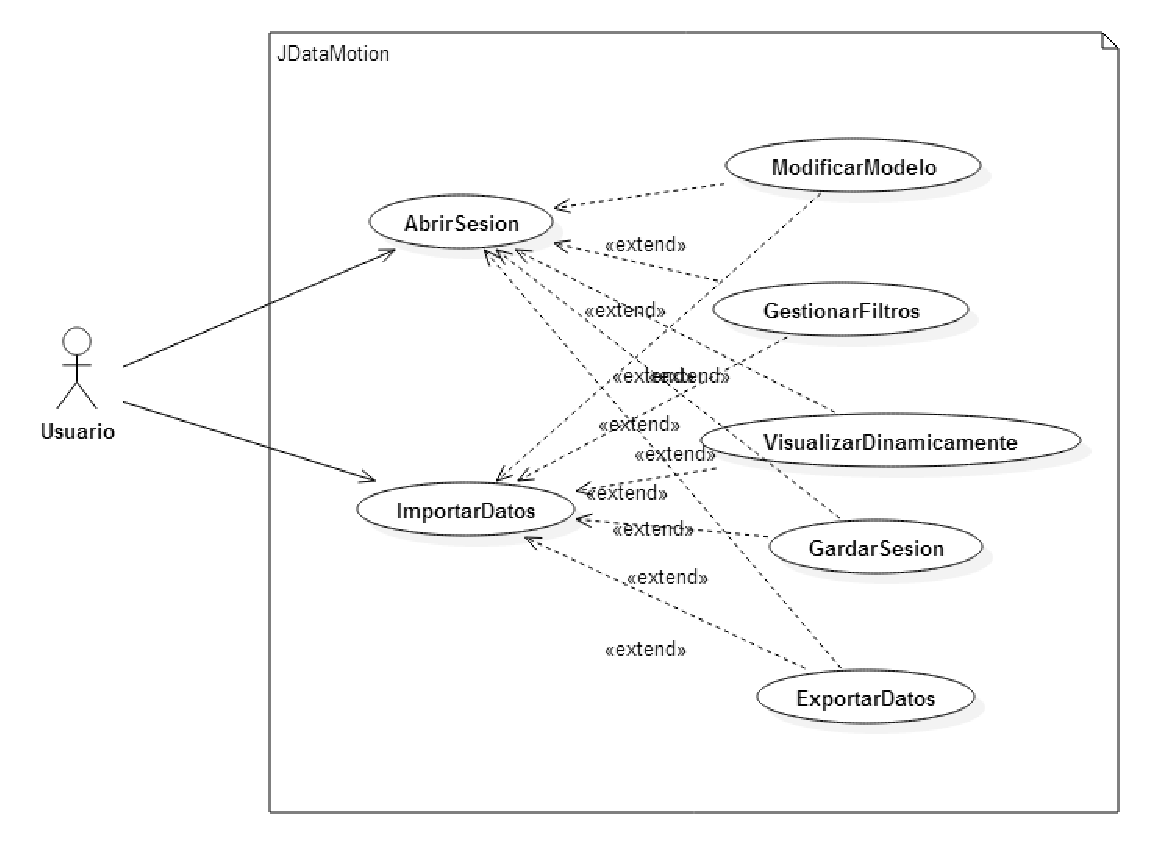
\includegraphics[width=\textwidth,height=\textheight,keepaspectratio]{figuras/casosUso}
\caption{Diagrama de casos de uso}
\label{casosUso}
\end{figure}

Un escenario de caso de uso podería comezar cun traballador do ámbito médico-sanitario que dispón nun csv (exportado por outra aplicación, por exemplo) de certas medicións relacionadas cun paciente seu ao longo do seu seguimento. O traballador (usuario do sistema) podería importar o arquivo dentro do JDataMotion e obter unha táboa editable cos datos contidos, aplicar filtros para eliminar os datos atípicos das medicións do paciente e normalizar algunhas variables. Cos datos xa preprocesados, poderá reproducilos para ver o seu comportamento ao longo do tempo e a evolución do paciente. Finalmente, gardará os datos filtrados baixo un novo csv.

\section{Requisitos funcionais}

\subsection*{RF01}
\begin{description}
\item[Título] \hfill \\
Importar arquivos con datos para o experimento
\item[Descrición] \hfill \\
A aplicación debe permitir cargar do sistema de arquivos un ficheiro que conteña unha secuencia de datos (nun formato axeitado segundo o RNF01) para ser utilizados no experimento.
\item[Importancia] \hfill \\
Esencial
\end{description}

\subsection*{RF02}
\begin{description}
\item[Título] \hfill \\
Exportar datos
\item[Descrición] \hfill \\
A aplicación debe permitir almacenar nun arquivo o conxunto de datos do experimento actual (tendo en conta filtrados, modificacións, datos engadidos ou eliminados...). Os arquivos de saída deberán respectar o RNF01 en canto a formato de almacenamento.
\subsubsection{Importancia}
Esencial
\end{description}

\subsection*{RF03}
\begin{description}
\item[Título] \hfill \\
Gardar sesión
\item[Descrición] \hfill \\
A aplicación debe permitir gardar en disco a sesión (ou experimento) actual tal e como está no momento de executar esta acción.
\item[Importancia] \hfill \\
Esencial
\end{description}

\subsection*{RF04}
\begin{description}
\item[Título] \hfill \\
Abrir sesión
\item[Descrición] \hfill \\
A aplicación debe permitir restaurar unha sesión (ou experimento) gardada anteriormente, de xeito que se atope exactamente igual ca no momento en que se gardou.
\item[Importancia] \hfill \\
Esencial
\end{description}

\subsection*{RF05}
\begin{description}
\item[Título] \hfill \\
Representar os datos en forma de táboa
\item[Descrición] \hfill \\
A aplicación debe ser capaz de amosar os datos segundo unha táboa na que figuren cabeceiras, tipos, valores, etc.
\item[Importancia] \hfill \\
Esencial
\end{description}

\subsection*{RF06}
\begin{description}
\item[Título] \hfill \\
Insertar datos no experimento actual
\item[Descrición] \hfill \\
A aplicación debe permitir a inserción dinámica de datos no experimento actual.
\item[Importancia] \hfill \\
Esencial
\end{description}

\subsection*{RF07}
\begin{description}
\item[Título] \hfill \\
Modificar datos no experimento actual
\item[Descrición] \hfill \\
A aplicación debe permitir a modificación dinámica de datos no experimento actual.
\item[Importancia] \hfill \\
Esencial
\end{description}

\subsection*{RF08}
\begin{description}
\item[Título] \hfill \\
Eliminar datos no experimento actual
\item[Descrición] \hfill \\
A aplicación debe permitir a eliminación dinámica de datos no experimento actual.
\item[Importancia] \hfill \\
Esencial
\end{description}

\subsection*{RF09}
\begin{description}
\item[Título] \hfill \\
Asignar tipos aos atributos dun arquivo importado
\item[Descrición] \hfill \\
A aplicación debe permitir especificar os tipos de atributos presentes no arquivo importado. Por exemplo, os datos cuantitativos poderían ser enteiros ou reais, mentres que os cualitativos serían algo distinto (mesmamente strings).
\item[Importancia] \hfill \\
Esencial
\end{description}

\subsection*{RF10}
\begin{description}
\item[Título] \hfill \\
Sinalar identificación temporal
\item[Descrición] \hfill \\
A aplicación debe permitir sinalar unha columna que exprese o orde ou a temporalidade dunha tupla, ou ben definir esta columna manualmente.
\item[Importancia] \hfill \\
Esencial
\end{description}

\subsection*{RF11}
\begin{description}
\item[Título] \hfill \\
Representar os datos graficamente mediante diagrama de dispersión
\item[Descrición] \hfill \\
A aplicación debe ser capaz de representar graficamente (mediante diagrama de dispersión) o conxunto de parámetros de entrada. Concretamente, débense poder representar ata 3 parámetros por cada diagrama de dispersión (ordeadas, abscisas e cor e forma dos puntos). Todos os diagramas de dispersión estarán englobados dentro do ``menú de visualización'', que cumprirá co RNF06.
\item[Importancia] \hfill \\
Esencial
\end{description}

\subsection*{RF12}
\begin{description}
\item[Título] \hfill \\
Engadir diagramas de dispersión ao menú de visualización
\item[Descrición] \hfill \\
A aplicación debe permitir engadir dinámicamente novos diagramas de dispersión dentro do menú de visualización.
\item[Importancia] \hfill \\
Esencial
\end{description}

\subsection*{RF13}
\begin{description}
\item[Título] \hfill \\
Eliminar un diagrama de dispersión do menú de visualización
\item[Descrición] \hfill \\
A aplicación debe permitir eliminar un diagrama de dispersión do menú de visualización.
\item[Importancia] \hfill \\
Esencial
\end{description}

\subsection*{RF14}
\begin{description}
\item[Título] \hfill \\
Configurar diagramas de dispersión do menú de visualización
\item[Descrición] \hfill \\
A aplicación debe permitir especificar para os diagramas de dispersión do menú de visualización a súa configuración, respecto a que parámetros se representarán en cada un dos eixos ou si as cores e formas dos puntos se desexan usar para representar algún atributo nominal.
\item[Importancia] \hfill \\
Esencial
\end{description}

\subsection*{RF15}
\begin{description}
\item[Título] \hfill \\
Detallar punto seleccionado dentro do diagrama de dispersión
\item[Descrición] \hfill \\
Cada punto dos diagramas de dispersión pode ser seleccionado para ver nun apartado os seus detalles (todos os seus atributos).
\item[Importancia] \hfill \\
Esencial
\end{description}

\subsection*{RF16}
\begin{description}
\item[Título] \hfill \\
Resaltar punto en diagramas de dispersión
\item[Descrición] \hfill \\
Cada punto seleccionalo dentro dun diagrama de dispersión resaltarase tanto nel coma en todos os demais diagramas de dispersión (que plasmarán outras proxeccións do mesmo punto).
\item[Importancia] \hfill \\
Esencial
\end{description}

\subsection*{RF17}
\begin{description}
\item[Título] \hfill \\
Desprazar a ventá de visualización por arrastre de cada diagrama de dispersión
\item[Descrición] \hfill \\
Para cada diagrama de dispersión poderemos usar unha ferramenta ``man'' para desprazar a ventá polo diagrama de dispersión.
\item[Importancia] \hfill \\
Esencial
\end{description}

\subsection*{RF18}
\begin{description}
\item[Título] \hfill \\
Escalar a ventá de visualización de cada diagrama de dispersión
\item[Descrición] \hfill \\
Para cada diagrama de dispersión poderemos usar unha ferramenta de escalado da ventá para facer zoom no diagrama de dispersión.
\item[Importancia] \hfill \\
Esencial
\end{description}

\subsection*{RF19}
\begin{description}
\item[Título] \hfill \\
Escalar e reposicionar dinamicamente
\item[Descrición] \hfill \\
Para cada diagrama de dispersión permitirase que a ventá de visualización que o enfoca se adapte dinamicamente ao conxunto de datos representados (movéndose, afastándose e aproximándose para englobar todos os datos).
\item[Importancia] \hfill \\
Esencial
\end{description}

\subsection*{RF20}
\begin{description}
\item[Título] \hfill \\
Reproducir a secuencia de datos
\item[Descrición] \hfill \\
A aplicación debe de permitir que a visualización dos diagramas de dispersión poida basearse na variable temporal (ou de orde) para reproducir a secuencia de datos, amosando os datos de cada diagrama de dispersión baixo unha secuencia de vídeo. Nesta secuencia engadiríase á visualización en cada instante a tupla de atributos asociada a esa marca temporal. 
\item[Importancia] \hfill \\
Esencial
\end{description}

\subsection*{RF21}
\begin{description}
\item[Título] \hfill \\
Representar estela
\item[Descrición] \hfill \\
A aplicación debe de permitir que cada novo punto pintado se ligue ao último representado no diagrama de dispersión por medio dunha liña recta.
\item[Importancia] \hfill \\
Esencial
\end{description}

\subsection*{RF22}
\begin{description}
\item[Título] \hfill \\
Difuminar estela ao longo da reprodución
\item[Descrición] \hfill \\
A aplicación debe permitir difuminar as estelas xa representadas a través do avance temporal.
\item[Importancia] \hfill \\
Esencial
\end{description}

\subsection*{RF23}
\begin{description}
\item[Título] \hfill \\
Configurar a reprodución da secuencia de datos
\item[Descrición] \hfill \\
A aplicación debe de permitir que a visualización dos diagramas de dispersión sexa configurable en canto a tempo transcorrido entre marcas temporais. Para a reprodución usando marcas temporais ponderadas, este tempo representará a separación entre as dúas marcas temporais mais próximas (tempo mínimo). Ademáis débese poder especificar o número de marcas temporais que durará o difuminado dos puntos que se ploteen, de xeito que durante ese intervalo cada punto se vaia difuminando ata desaparecer. Pode ser igual a 0 para que os puntos non se difuminen.
\item[Importancia] \hfill \\
Esencial
\end{description}

\subsection*{RF24}
\begin{description}
\item[Título] \hfill \\
Pausar a reprodución
\item[Descrición] \hfill \\
A aplicación debe permitir parar a reprodución na marca de tempo na que se atope ao executar esta acción, mantendo as visualizacións para ese momento.
\item[Importancia] \hfill \\
Esencial
\end{description}

\subsection*{RF25}
\begin{description}
\item[Título] \hfill \\
Ir a un determinado instante dentro do intervalo temporal da reprodución
\item[Descrición] \hfill \\
A aplicación debe permitir situarse directamente sobre un instante de tempo, mantendo a reprodución pausada sobre esa marca temporal, e visualizando os diagramas de dispersión tal e como deben estar nese momento.
\item[Importancia] \hfill \\
Esencial
\end{description}

\subsection*{RF26}
\begin{description}
\item[Título] \hfill \\
Insertar filtros para os datos do experimento
\item[Descrición] \hfill \\
A aplicación debe permitir engadir unha serie de filtros que se aplicarán de xeito secuencial sobre a secuencia de datos coa que se esté a traballar. Chamarémoslle ``secuencia de filtros'' a esta secuencia.
\item[Importancia] \hfill \\
Esencial
\end{description}

\subsection*{RF27}
\begin{description}
\item[Título] \hfill \\
Eliminar un filtro para os datos do experimento
\item[Descrición] \hfill \\
A aplicación debe permitir eliminar un determinado filtro dentro da secuencia de filtros.
\item[Importancia] \hfill \\
Esencial
\end{description}

\subsection*{RF28}
\begin{description}
\item[Título] \hfill \\
Configurar filtros para os datos do experimento
\item[Descrición] \hfill \\
A aplicación debe permitir seleccionar un determinado filtro dentro da secuencia de filtros para modificar a regla de filtrado implícita.
\item[Importancia] \hfill \\
Esencial
\end{description}

\subsection*{RF29}
\begin{description}
\item[Título] \hfill \\
Gardar unha secuencia de filtros do experimento
\item[Descrición] \hfill \\
A aplicación debe permitir gardar unha secuencia de filtros, non necesariamente correlativos, dentro dos que se estean aplicando sobre o experimento. Esta secuencia pode comprender tanto un só filtro como a secuencia de filtros enteira.
\item[Importancia] \hfill \\
Esencial
\end{description}

\subsection*{RF30}
\begin{description}
\item[Título] \hfill \\
Cargar unha secuencia de filtros para o experimento
\item[Descrición] \hfill \\
A aplicación debe permitir cargar do sistema de arquivos unha secuencia de filtros que se engadirá á cabeza da secuencia de filtros (a cal pode estar baleira). Esta secuencia tamén pode estar composta por un só filtro.
\item[Importancia] \hfill \\
Esencial
\end{description}

\subsection*{RF31}
\begin{description}
\item[Título] \hfill \\
Mover os filtros dentro da secuencia de filtros
\item[Descrición] \hfill \\
A aplicación debe permitir desprazar un filtro dentro da secuencia de filtros do experimento, de xeito que o orde de aplicación dos filtros varíe. O desprazamento realizarase inserindo o filtro en cuestión nunha nova posición.
\item[Importancia] \hfill \\
Esencial
\end{description}

\subsection*{RF32}
\begin{description}
\item[Título] \hfill \\
Configurar o menú de visualización
\item[Descrición] \hfill \\
A aplicación debe permitir cambiar os parámetros de visualización dos diagramas de dispersión que compoñen o menú de visualización, por exemplo, a cor das etiquetas e lendas, do fondo, dos eixos... ou a fonte, tamaño de letra...
\item[Importancia] \hfill \\
Optativa
\end{description}

\section{Requisitos de calidade}

\subsection*{RC01}
\begin{description}
\item[Título] \hfill \\
Latencia mínima para o procesamento
\item[Descrición] \hfill \\
A aplicación debe responder nun tempo razoable ás operacións executadas polo usuario, e intentar que esa latencia escale de xeito controlado ao aumentar a talla dos parámetros.
\item[Importancia] \hfill \\
Esencial
\end{description}

\section{Requisitos de deseño}

\subsection*{RD01}
\begin{description}
\item[Título] \hfill \\
Modularidade no deseño dos filtros
\item[Descrición] \hfill \\
A aplicación debe facilitar unha interface para a inclusión e uso de filtros personalizados por parte de calquera desenvolvedor de software que a implemente dentro do proxecto.
\item[Importancia] \hfill \\
Esencial
\end{description}

\section{Requisitos non funcionais}

\subsection*{RNF01}
\begin{description}
\item[Título] \hfill \\
Formatos de arquivo admitidos ao importar e exportar arquivos
\item[Descrición] \hfill \\
A aplicación debe estar preparada para importar e exportar arquivos en distintos formatos, como son o CSV e ARFF.
\item[Importancia] \hfill \\
Esencial
\end{description}

\subsection*{RNF02}
\begin{description}
\item[Título] \hfill \\
Relación programa-sesión
\item[Descrición] \hfill \\
Cada instancia do programa debe traballar cunha única sesión (experimento).
\item[Importancia] \hfill \\
Esencial
\end{description}

\subsection*{RNF03}
\begin{description}
\item[Título] \hfill \\
Implementación en Java
\item[Descrición] \hfill \\
O software tense que desenvolver na linguaxe de programación Java.
\item[Importancia] \hfill \\
Esencial
\end{description}

\subsection*{RNF04}
\begin{description}
\item[Título] \hfill \\
Representación matricial dos diagramas de dispersión
\item[Descrición] \hfill \\
Os diagramas de dispersión represéntanse de xeito matricial, facendo que cada parámetro dentro dun eixo sexa enfrontado a cada un dos demais do outro eixo, e en cada punto desa dupla se sitúe o diagrama de dispersión que compara ambos parámetros. Deste xeito, os diagramas de dispersión non son acumulables: se temos un que representa X (abscisas) fronte a Y (ordenadas), non podemos engadir outro que represente X (abscisas) fronte a Y (ordenadas), pois ocuparían ambos a mesma cela dentro da matriz de diagramas de dispersión.
\item[Importancia] \hfill \\
Esencial
\end{description}

\subsection*{RNF05}
\begin{description}
\item[Título] \hfill \\
Entrega dentro de prazo
\item[Descrición] \hfill \\
Débese entregar unha versión funcional e documentada antes do día 13 de Febreiro de 2014, ás 14:00 horas, pois é o momento no que remata o prazo de entrega.
\item[Importancia] \hfill \\
Esencial
\end{description}

\section{RFs dos sprints}

Imos a detallar a asignación de requisitos funcionais (RFs) aos distintos sprints ao longo da fase de Desenvolvemento, asignando uns prazos aproximados de traballo sobre uns conxunto de RFs relacionados entre si.

\subsection*{Sprint 01}
\begin{description}
\item[Nome:] Interacción co sistema de ficheiros
\item[Fase:] Desenvolvemento
\item[Comezo:] 17/02/2014
\item[Finalización:] 24/02/2014
\item[RFs a implementar:] RF01, RF02, RF03, RF04
\end{description}

\subsection*{Sprint 02}
\begin{description}
\item[Nome:] Manipulación de datos
\item[Fase:] Desenvolvemento
\item[Comezo:] 24/02/2014
\item[Finalización:] 10/03/2014
\item[RFs a implementar:] RF05, RF06, RF07, RF08
\end{description}

\subsection*{Sprint 03}
\begin{description}
\item[Nome:] Preprocesado
\item[Fase:] Desenvolvemento
\item[Comezo:] 10/03/2014
\item[Finalización:] 24/03/2014
\item[RFs a implementar:] RF09, RF10
\end{description}

\subsection*{Sprint 04}
\begin{description}
\item[Nome:] Visualización dos datos
\item[Fase:] Desenvolvemento
\item[Comezo:] 24/03/2014
\item[Finalización:] 14/04/2014
\item[RFs a implementar:] RF11, RF12, RF13, RF14
\end{description}

\subsection*{Sprint 05}
\begin{description}
\item[Nome:] Ferramentas de visualización
\item[Fase:] Desenvolvemento
\item[Comezo:] 14/04/2014
\item[Finalización:] 28/04/2014
\item[RFs a implementar:] RF15, RF16, RF17, RF18, RF19
\end{description}

\subsection*{Sprint 06}
\begin{description}
\item[Nome:] Reprodución
\item[Fase:] Desenvolvemento
\item[Comezo:] 28/04/2014
\item[Finalización:] 05/05/2014
\item[RFs a implementar:] RF20
\end{description}

\subsection*{Sprint 07}
\begin{description}
\item[Nome:] Configuración da reprodución
\item[Fase:] Desenvolvemento
\item[Comezo:] 05/05/2014
\item[Finalización:] 19/05/2014
\item[RFs a implementar:] RF21, RF22, RF23
\end{description}

\subsection*{Sprint 08}
\begin{description}
\item[Nome:] Funcións de reprodución
\item[Fase:] Desenvolvemento
\item[Comezo:] 19/05/2014
\item[Finalización:] 02/06/2014
\item[RFs a implementar:] RF24, RF25
\end{description}

\subsection*{Sprint 09}
\begin{description}
\item[Nome:] Filtros
\item[Fase:] Desenvolvemento
\item[Comezo:] 02/06/2014
\item[Finalización:] 16/06/2014
\item[RFs a implementar:] RF26, RF27, RF28
\end{description}

\subsection*{Sprint 10}
\begin{description}
\item[Nome:] Xestionar filtros
\item[Fase:] Desenvolvemento
\item[Comezo:] 16/06/2014
\item[Finalización:] 30/06/2014
\item[RFs a implementar:] RF29, RF30, RF31
\end{description}

\subsection*{Sprint 11}
\begin{description}
\item[Nome:] Outras funcións de visualización
\item[Fase:] Desenvolvemento
\item[Comezo:] 30/06/2014
\item[Finalización:] 07/07/2014
\item[RFs a implementar:] RF32
\end{description}

A partir da planificación temporal de grupos de RFs en común podemos estimar con certa confianza a duración total do proxecto, polo menos na súa fase de desenvolvemento. Faltarían dúas fases máis por considerar:

\begin{itemize}
\item Fase de inicio, previa á execución dos sprints, duraría un prazo de 2 semanas e constaría das seguintes tarefas:
\begin{itemize}
\item Lectura da especificación e documentación
\item Reunión cos directores do proxecto
\item Redacción do anteproxecto
\end{itemize} 
\item Fase de documentación, posterior á execución dos sprints, duraría un prazo de 5 semanas e constaría das seguintes tarefas:
\begin{itemize}
\item Revisión e documentación do código
\item Compilación de documentos cos sprints
\item Redacción da memoria
\item Redacción dun manual de usuario
\item Reunión co director para revisión
\end{itemize}
\end{itemize} 

Agora que temos as estimacións da fase de inicio, da fase de documentación e da fase de desenvolvemento (cos seus sprints estimados) podemos realizar un diagrama de Gantt do proxecto (figura \ref{gantt}) para establecer a liña base do mesmo:

\begin{figure}
\centering
\includegraphics[width=\textwidth,height=\textheight,keepaspectratio]{figuras/gantt}
\caption{Diagrama de Gantt}
\label{gantt}
\end{figure}

Considerando que coñecemos as tarefas da fase de inicio e da fase de documentación, así como os sprints da fase de desenvolvemento e incluso os RFs a desenvolver dentro de cada un deles, podemos plasmar todas estas tarefas nun Esquema de Descomposición do Traballo ou EDT (figura \ref{edt}). Isto implica que os RFs (ou máis ben o seu desenvolvemento) van ter a consideración de tarefas a partir de agora no noso proxecto.

\begin{figure}
\centering
\includegraphics[width=\textwidth,height=\textheight,keepaspectratio]{figuras/edt}
\caption{Esquema de Descomposición do Traballo (EDT)}
\label{edt}
\end{figure}

\chapter{Análise de tecnoloxías}

Chegados a este punto, temos un conxunto de tarefas especificadas e delimitadas no tempo que se van realizar, así que agora abordaremos as tecnoloxías (ferramentas e técnicas) que imos utilizar para levalas a cabo.

\section{Arquitectura}

Nesta sección imos comentar a arquitectura sobre a que estará cimentada o noso proxecto. É importante considerar á hora de elixila que a nosa aplicación non só debe funcionar correctamente con ela, se non que ademais debe facilitar a súa mellora e evolución ao longo do tempo, ou o que é o mesmo, debe permitir a súa escalabilidade.

Na especificación deste proxecto e na captura de requisitos falouse do JDataMotion como unha ferramenta que permite visualizar dinamicamente conxuntos de datos que o usuario aporta. Esta premisa xa nos permite entrever que o modelo de datos non ten necesidade de ser extraido da máquina do cliente. Pódese traballar sobre ela de xeito local e obter resultados (visuais, ou un novo ficheiro de información procesada) sen necesidade de interactuar con sistemas externos (o que sería a computación distribuída). A arquitectura elixida será, segundo estas premisas, a dunha aplicación de escritorio.

\section{Tecnoloxías}

A partir do paradigma de computación que escollemos hai que elixir un conxunto de tecnoloxías que non só sexan compatibles con ela, se non que ademais permitan desenvolver satisfactoriamente os RFs pactados.

\subsection{Ferramentas de deseño}

\subsubsection{UML}

UML (Unified Modeling Language) é un estándar de modelado perfectamente aplicable ao un entorno de desenvolvemento de software. Baséase na especificación e documentación dos compoñentes do sistema a diferentes niveis, dentro da fase de deseño do sistema. Nós empregaremos este estándar mediante 3 tipos de diagramas:

\begin{description}
\item[Diagramas de casos de uso:] Na figura \ref{casosUso} xa presentamos o diagrama de casos de uso do sistema.
\item[Diagrama de clases:] Este tipo de diagrama presenta as clases que subxacen baixo o sistema, xunto cos seus métodos, atributos e interrelacións.
\item[Diagramas de secuencia:] Estes diagramas plasman a interacción entre os compoñentes (ou obxectos) do sistema durante escenarios concretos da execución da aplicación. Neles amósase o intercambio de información e o fluxo de control entre compoñentes.
\end{description} 

\subsection{Ferramentas de desenvolvemento}

A única imposición a nivel de desenvolvemento dada pola especificación do anteproxecto é perfectamente válida coas premisas tomadas ata agora: o sistema debe ser implementado na linguaxe de programación Java.

\subsubsection{Java}

Java é unha linguaxe de programación de propósito xeral, é dicir, contén librarías e soporte para diversos propósitos: acceso a base de datos, comunicación entre máquinas, cálculo matemático, procesamento de imaxes, etc. Tamén é unha linguaxe concorrente, pois contén fornecemento para fíos de execución que van dan lugar, entre outras moitas vantaxes, á posibilidade de crear unha interface gráfica como a que imos necesitar.

Outras vantaxes que Java nos ofrece implicitamente son as seguintes:

\begin{itemize}
\item Java é multiplataforma, é dicir, o código que se programa compílase unha soa vez para ser empregado en calquera sistema, sen importar a súa especificación (sistema operativo, arquitectura do computador, etc.).
\item O colector de lixo, que nos permite abstraernos do proceso de liberación de recursos na memoria. Este sistema localiza e libera automaticamente na memoria aqueles obxectos que deixaron de ser referenciados (e polo tanto xa non vai volver a empregar o programa).
\end{itemize} 

Java é unha das linguaxes máis populares para practicar a programación orientada a obxectos. Este paradigma, que traballa con clases e obxectos para modelar entidades reais como van ser as táboas, os filtros e por suposto os diagramas de dispersión, está particularmente ben adaptado para traballar coas interfaces gráficas. Outras vantaxes da programación orientada a obxectos das que nos imos beneficiar son a herdanza, o encapsulamento e o polimorfismo.

Para o noso proxecto, a versión de Java que imos empregar vai ser a 8, en calquera das súas actualizacións (1.8.X, sendo X calquer valor). Para a execución do JDataMotion deberemos ter instalada unha versión igual ou superior da máquina virtual de Java, que podemos descargar dende o sitio web oficial \cite{java}.

\subsubsection{JFreeChart}

Na especificación do proxecto tamén se deixa caer unha decisión que afectará significativamente ao desenvolvemento do proxecto cerca das últimas tarefas deste (sprints asociados a visualización dos datos) e é o de elixir unha libraría gráfica axeitada para as nosas necesidades á hora de representar os diagramas de dispersión.

Facendo un balance das principais solucións que existen actualmente na web, obtivemos:

\begin{itemize}
\item JFreeChart
\item JZY3D
\item Project Waterloo
\item GRAL
\item JChart2D
\item JenSoft Java Chart API
\item JRobin
\end{itemize} 

Deste conxunto saleu como mellor posicionado o proxecto JFreeChart \cite{jfreechart} de acordo ás seguintes características:

\begin{itemize}
\item É a solución que conta cun soporte máis activo. JFreeChart parecía ser o único proxecto no momento de tomar esta decisión que seguía sacando novas versións, actualizacións e parches. A solución JZY3D, sendo a segunda máis recente, non sacou unha nova versión dende o 2013, e no caso de JRobin a última versión é do 2011. Tendo en conta que Java 8 foi liberado en Marzo do 2014, parece ser que só JFreeChart se fixo eco da aparición da nova versión da máquina virtual, e polo tanto é a única librería que lle estará sacando partido a estas melloras.
\item Non só é unha solución de software libre, senón que ademais é de código aberto. Isto será determinante á hora de acceder aos métodos e clases da librería, pois deberemos sobrescribir algúns para que se adecúen ao noso proxecto. De todos xeitos, as demais solucións presentadas tamén debían reunir esta característica á hora de ser elixidas.
\item A documentación de JFreeChart é moi completa, os Javadocs da súa interface de programación de aplicacións (API) explican perfectamente a funcionalidade da librería, co que se reducen os custes temporais de aprendizaxe.
\item O seu deseño favorece a herdanza de clases en beneficio das necesidades do noso proxecto.
\item Incorpora as funcións de configuración gráfica necesarias no que atinxe aos diagramas de dispersión. Por medio de menús contextuais, cada diagrama de dispersión pode fixar a cor de fondo, títulos e eixos, ou a fonte e tamaño de letra das etiquetas por exemplo. Tamén pode exportar en distintos formatos de imaxe o diagrama en cuestión, copialo ao portapapeis.
\item Permite a adición dinámica de puntos ao diagrama de dispersión. Isto será clave no proceso de reprodución dos datos.
\item Incorpora as funcións de axuste da ventá de visualización para os diagramas de dispersión. Cada vez que creemos un diagrama de dispersión, este xa contará coa posibilidade de ser desprazado ou escalado dentro da súa ventá de visualización. Ademais tamén mellora a inserción dinámica de puntos no diagrama, pois cada vez que un punto se engade ao diagrama, a ventá reposiciónase para seguir abarcando todos os puntos.
\end{itemize} 

\subsubsection{JCommon}

JCommon é unha librería da cal depende JFreeChart. Temos que acoplala ao proxecto, pero non imos ter necesidade de utilizala directamente.

\subsubsection{Formatos de arquivo}

No RNF01 fálase de dous tipos de arquivo de entrada e saída: ``csv'' e ``arff''.

O formato csv (comma-separated values) de arquivos almacena os datos dun xeito tabular simple. A primeira liña dun arquivo csv contén separados por N-1 comas os N nomes dos atributos ou columnas da táboa (se segue o estándar). A continuación, cada nova liña conterá tamén N-1 comas para separar os N valores que toma esa entrada para cada atributo. Un valor nulo represéntase deixando baleiro o oco correspondente.

O formato arff \bibitem{arff} é un formato de arquivo que contén a mesma información ca o csv, pero a maiores especifica o tipo de valores que se admiten para cada atributo, e tamén o nome da relación. A estrutura desta información é a seguinte:

\begin{description}
\item[@RELATION <nome da relación>] só unha vez en cada arquivo, sinala o nome da relación contida no ficheiro.
\item[@ATTRIBUTE <nome dun atributo> <tipo do atributo>] incluirase unha entrada coma esta por cada atributo da relacion. O tipo do atributo pode ser un dos seguintes:
\begin{itemize}
\item numeric (atributo numérico)
\item \textless valor nominal 1, valor nominal 2, valor nominal 3, ...\textgreater (atributo nominal, é dicir, que só pode tomar un dos valores nominais especificados na lista)
\item string (calquera cadea de caracteres)
\item date [\textless formato de data\textgreater ] (data no formato dado)
\end{itemize} 
\item[@DATA \textbackslash n \textless entrada 1 \textbackslash n entrada 2 \textbackslash n entrada 3 \textbackslash n ...\textgreater] despois de poñer a cláusula @DATA, engadirase unha nova liña para cada entrada. En cada entrada figurarán separados por comas os valores que esta toma para cada atributo (igual ca nos csv). Cada un desos valores asóciase ao atributo declarado na mesma posición.
\item[\% \textless calquera liña de texto \textgreater] os comentarios comezan co símbolo '\%' e abranguen a liña enteira. Poden ir intercalados en calquera zona do ficheiro.
\end{description} 

\subsubsection{Weka}

A raíz da documentación atopada sobre o formato arff vimos mencionado varias veces o término Weka. Weka (Waikato Environment for Knowledge Analysis) é unha plataforma de software libre para o aprendizaxe automático e a minería de datos, desenvolvido en Java pola Universidade de Waikato. Esta universidade precisamente creou o formato arff para Weka.

O software de Weka pódese obterse a través do seu sitio web \cite{weka}. A apariencia do programa tras importar un arquivo arff pódese observar na figura \ref{weka}, e na figura \ref{wekaDiagramas} podemos observar como Weka plasma os datos do arquivo baixo unha matriz de diagramas de dispersión. Como se pode ver, Weka xa realiza as funcións de importación e visualización dos datos.

\begin{figure}
\centering
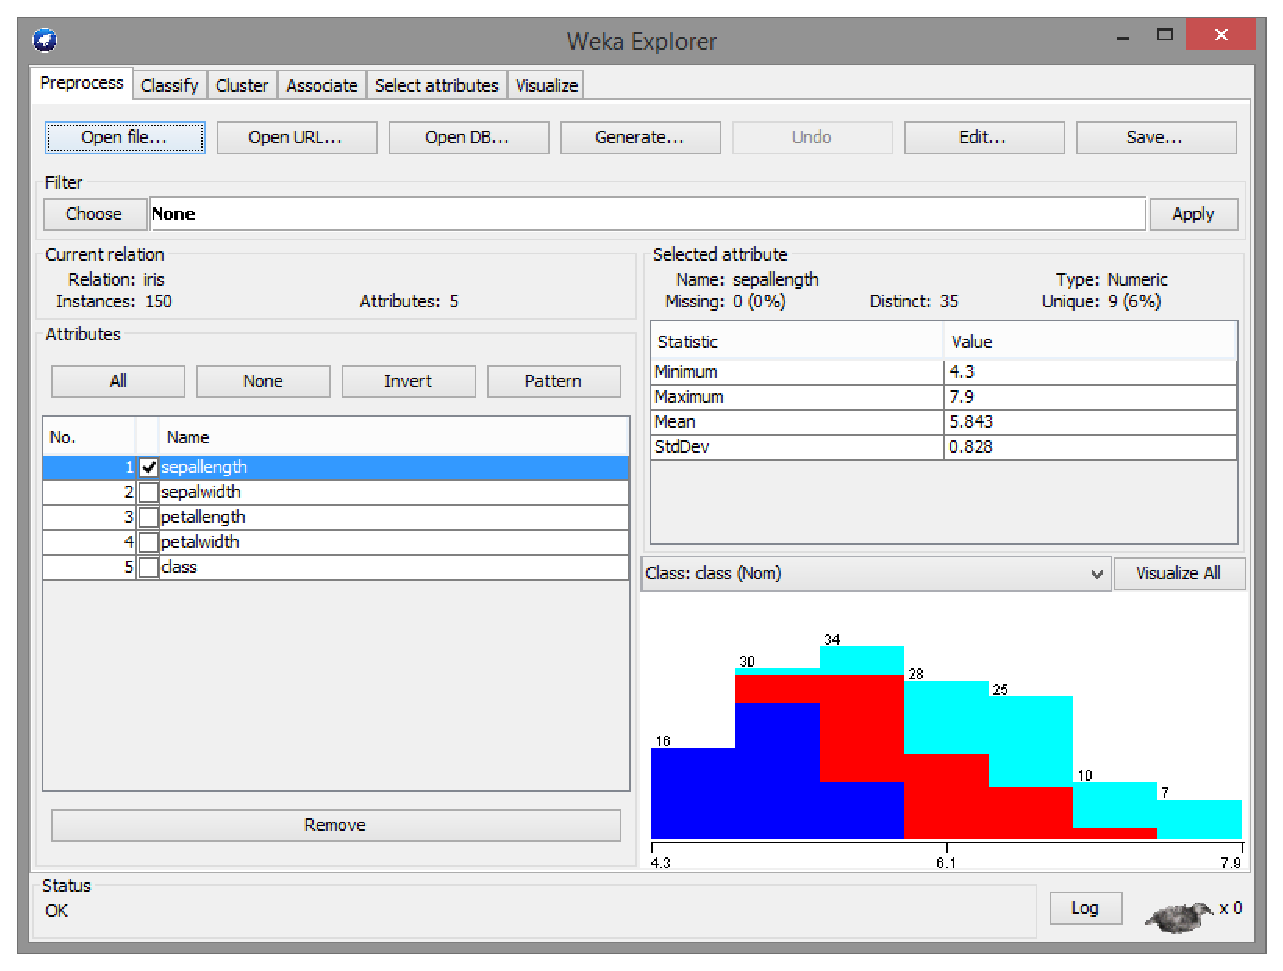
\includegraphics[width=\textwidth,height=\textheight,keepaspectratio]{figuras/weka}
\caption{Software Weka}
\label{weka}
\end{figure}

\begin{figure}
\centering
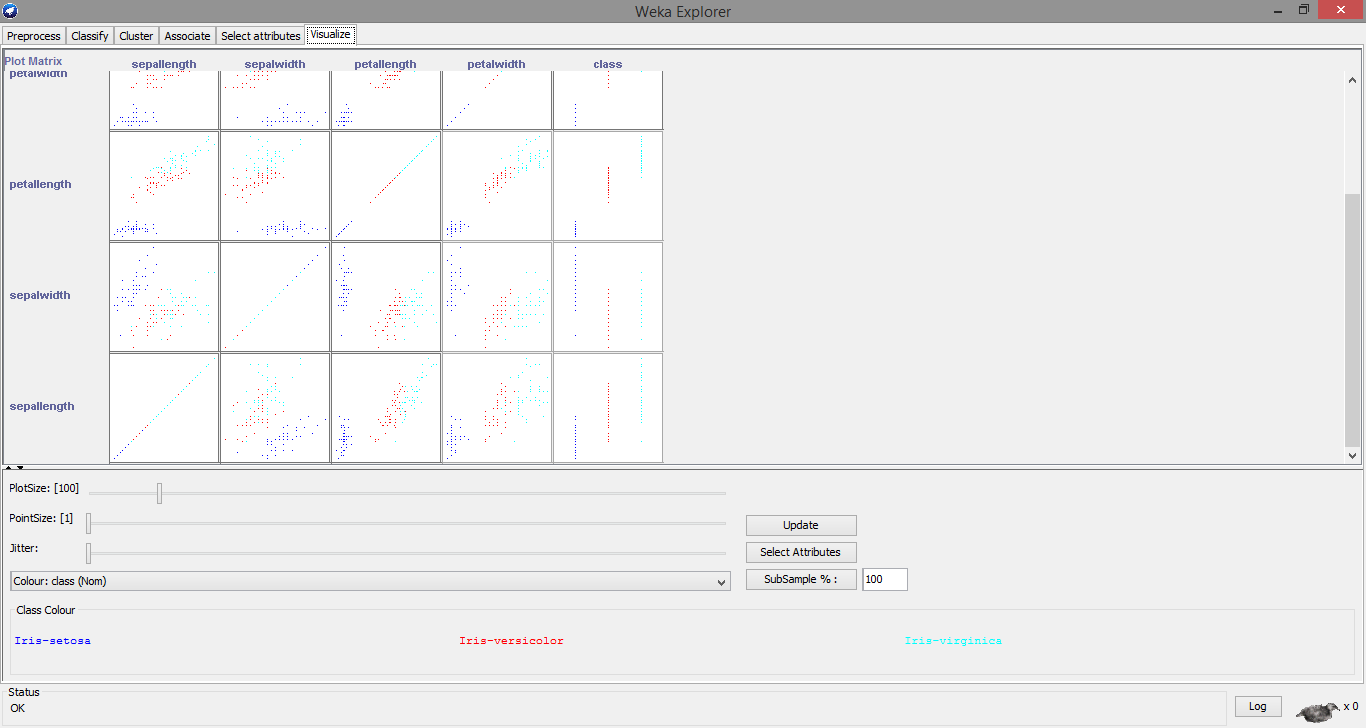
\includegraphics[width=\textwidth,height=\textheight,keepaspectratio]{figuras/wekaDiagramas}
\caption{Diagramas de dispersión en Weka}
\label{wekaDiagramas}
\end{figure}

Podemos extraer de Weka non só ideas para a interface do JDataMotion e das súas funcionalidades, se non que ademais, gracias a que Weka é un proxecto de código aberto, poderemos reutilizar o proxecto como unha libraría mais, utilizando os métodos e clases públicas que ofrece a súa interface de programación (API) para implementar facilmente a importación dos datos desde arquivo. A visualización dos datos tamén podería ser reutilizada, pero os diagramas de dispersión de Weka son estáticos, e a súa solución de visualización non vai servir para o JDataMotion. Weka non implementa a reprodución da visualización que JDataMotion busca.

\subsubsection{Swing}

Swing é unha libraría gráfica expresamente deseñada para Java. Inclúe unha serie de elementos (coñecidos como ``widgets'') para facilitar a confección da interface gráfica a calquera desenvolvedor. Ao igual que Java, Swing é independente da plataforma, e ademáis posibilita en gran medida e extensión de clases, ou widgets, para adaptalos ás necesidades de calquera interface gráfica.

\subsubsection{NetBeans IDE}

NetBeans IDE é un entorno de desenvolvemento integrado, especialmente deseñado para programar sistemas en linguaxe Java, aínda que tamén da soporte a moitos outros linguaxes de programación. En NetBeans poderemos programar con facilidade as clases que logo o IDE compilará e executará. Tamén facilitará as labores de adxuntar librarías e dependencias, e dará fornecemento ao deseño da interface por medio dun lenzo e unha paleta de ``widgets'' propios de Swing, o cal reducirá o tempo que tardemos en aprender a manexar a libraría Swing.

\subsection{Ferramentas de validación}

A validación é un proceso que permite contrastar os resultados da implementación do sistema fronte aos requisitos (funcionais, non funcionais, de deseño, de calidade, etc) que inicialmente se esperaban dela.

\subsubsection{JUnit}

JUnit \cite{junit} é un compendio de librarías para aplicacións Java destinadas a realizar probas unitarias do sistema no que se inclúen. Contén un conxunto de clases que actúan sobre as clases e métodos do sistema orixinal, validando a súa resposta ante certos parámetros de entrada.